\documentclass[11pt,a4paper,spanish]{book}
\usepackage{estilo_unir-1}
\hypersetup{
	colorlinks   = true,
	urlcolor     = blue,
	linkcolor    = black,
	citecolor    = red
}
\usepackage[nottoc]{tocbibind}
\usepackage{longtable}
\usepackage{booktabs}
\usepackage{array}
\usepackage{tikz}
\usetikzlibrary{arrows.meta, positioning}

%---------------------------
% Datos del trabajo
%---------------------------
\subject{Pr\'{a}cticas Acad\'{e}micas Externas}
\title{Sistema de medici\'{o}n de impedancia (EIS) para cuantificaci\'{o}n de Candida albicans --- Cronograma de trabajo}
\author{Andr\'{e}s Alexandro Tapia Flores}
\profesor{Universidad Internacional de la Rioja (UNIR)}
\date{Mayo 2026}

\begin{document}
\renewcommand{\listtablename}{\'{I}ndice de tablas}
\renewcommand{\contentsname}{\'{I}ndice de contenidos}
\renewcommand{\tablename}{Tabla}
\setlength{\headheight}{26pt}

\maketitle
\frontmatter
\tableofcontents

\mainmatter

\chapter{Cronograma de trabajo}

Este documento presenta el cronograma detallado del trabajo realizado durante las pr\'{a}cticas acad\'{e}micas externas, desde la reuni\'{o}n de bienvenida (17 de marzo de 2026) hasta la entrega final (20 de mayo de 2026). Se indican las actividades principales de cada semana, las reuniones con el tutor y los entregables producidos.

\section{Calendario de reuniones}

Las reuniones con el tutor se realizaron de forma recurrente cada mi\'{e}rcoles, comenzando el 25 de marzo de 2026. La Tabla~\ref{tab:reuniones} resume las fechas de las reuniones y los temas tratados.

\begin{table}[ht]
\centering
\begin{tabular}{c l p{9cm}}
\hline\hline
No. & Fecha & Tema tratado \\ [0.5ex]
\hline
-- & 17 mar 2026 & Reuni\'{o}n de bienvenida al proyecto de pr\'{a}cticas. Presentaci\'{o}n del proyecto, alcance y objetivos generales. \\ \hline
1 & 25 mar 2026 & Primera reuni\'{o}n con el tutor. Revisi\'{o}n del documento inicial. Cambio de tecnolog\'{i}a: de LabVIEW a Python + React. Redefinici\'{o}n de la arquitectura del sistema y las variables EIS. Acuerdos sobre las fases del desarrollo. \\ \hline
2 & 1 abr 2026 & Seguimiento de la Fase~1. Revisi\'{o}n de la especificaci\'{o}n de requerimientos funcionales (RF-01 a RF-09). Definici\'{o}n del diagrama de bloques del sistema. \\ \hline
3 & 8 abr 2026 & Cierre de la Fase~1 y entrega del Entregable~1. Inicio de la Fase~2: protocolo de comunicaci\'{o}n Python--ESP32. Primer commit del repositorio. \\ \hline
4 & 15 abr 2026 & Avance de la Fase~2. Revisi\'{o}n de los comandos implementados (PING, CFG, CAL, START, STOP, TEMP). Discusi\'{o}n del enfoque de clasificaci\'{o}n cu\'{a}ntica variacional (VQC). \\ \hline
5 & 22 abr 2026 & Cierre de la Fase~2. Avance de las Fases~3 y 4: tarjeta simulada, backend WebSocket, dashboard React. Integraci\'{o}n del clasificador cu\'{a}ntico-cl\'{a}sico. \\ \hline
6 & 29 abr 2026 & Cierre de las Fases~3 y 4. Modelo de sesi\'{o}n persistente, exportaci\'{o}n multi-formato, validaci\'{o}n de latencias. Diagrama esquem\'{a}tico de conexi\'{o}n del sistema. \\ \hline
7 & 6 may 2026 & Inicio de la Fase~5. Planificaci\'{o}n del reporte t\'{e}cnico, manual de usuario y documentaci\'{o}n final. \\ \hline
8 & 13 may 2026 & Avance de la Fase~5. Captura automatizada de pantallas del dashboard. Revisi\'{o}n de la secci\'{o}n de computaci\'{o}n cu\'{a}ntica aplicada y an\'{a}lisis de repetibilidad. \\ \hline
9 & 20 may 2026 & Entrega final. Revisi\'{o}n y cierre de la memoria, manual de usuario y cronograma. \\ \hline
\end{tabular}
\caption[Calendario de reuniones]{Calendario de reuniones con el tutor y eventos clave del proyecto. Fuente: elaboraci\'{o}n propia.}
\label{tab:reuniones}
\end{table}

\section{Detalle semana a semana}

\subsection{Semana 1: 17--23 de marzo de 2026}

\begin{table}[ht]
\centering
\begin{tabular}{p{3cm} p{10cm}}
\hline\hline
\textbf{Periodo} & 17--23 de marzo de 2026 \\ [0.5ex]
\hline
\textbf{Fase} & Preparaci\'{o}n \\ \hline
\textbf{Actividades} & Reuni\'{o}n de bienvenida al proyecto de pr\'{a}cticas (17 de marzo). Presentaci\'{o}n del proyecto de desarrollo de un sistema EIS para cuantificaci\'{o}n de \textit{Candida albicans}. Revisi\'{o}n del documento inicial que propon\'{i}a LabVIEW como entorno de desarrollo. Configuraci\'{o}n del entorno de trabajo y acceso a los recursos del proyecto. \\ \hline
\textbf{Entregable} & Ninguno \\ \hline
\end{tabular}
\caption[Semana 1]{Detalle de la Semana~1. Fuente: elaboraci\'{o}n propia.}
\label{tab:semana1}
\end{table}

\subsection{Semana 2: 24--30 de marzo de 2026}

\begin{table}[ht]
\centering
\begin{tabular}{p{3cm} p{10cm}}
\hline\hline
\textbf{Periodo} & 24--30 de marzo de 2026 \\ [0.5ex]
\hline
\textbf{Fase} & Fase~1 --- An\'{a}lisis del sistema y definici\'{o}n de requerimientos \\ \hline
\textbf{Actividades} & Primera reuni\'{o}n con el tutor (25 de marzo). Decisi\'{o}n clave: migrar de LabVIEW a una implementaci\'{o}n opensource en Python y React, por mayor portabilidad, integraci\'{o}n con bibliotecas de an\'{a}lisis de datos y computaci\'{o}n cu\'{a}ntica. Redefinici\'{o}n de la arquitectura del sistema: ESP32 + AD5933 (hardware), Python backend (software), React frontend (visualizaci\'{o}n). Identificaci\'{o}n de las variables EIS: frecuencia, $\mathrm{Re}(Z)$, $\mathrm{Im}(Z)$, $|Z|$, fase, temperatura. \\ \hline
\textbf{Entregable} & Ninguno \\ \hline
\end{tabular}
\caption[Semana 2]{Detalle de la Semana~2. Fuente: elaboraci\'{o}n propia.}
\label{tab:semana2}
\end{table}

\subsection{Semana 3: 31 de marzo -- 6 de abril de 2026}

\begin{table}[ht]
\centering
\begin{tabular}{p{3cm} p{10cm}}
\hline\hline
\textbf{Periodo} & 31 de marzo -- 6 de abril de 2026 \\ [0.5ex]
\hline
\textbf{Fase} & Fase~1 --- An\'{a}lisis del sistema y definici\'{o}n de requerimientos \\ \hline
\textbf{Actividades} & Reuni\'{o}n con el tutor (1 de abril). Elaboraci\'{o}n de los nueve requerimientos funcionales (RF-01 a RF-09). Dise\~{n}o del diagrama de bloques del sistema con las tres capas (hardware, backend, frontend). An\'{a}lisis del protocolo de comunicaci\'{o}n serial ESP32--PC. Documentaci\'{o}n de la especificaci\'{o}n de la tarjeta EVAL-AD5940ELCZ y el AD5933. \\ \hline
\textbf{Entregable} & Ninguno \\ \hline
\end{tabular}
\caption[Semana 3]{Detalle de la Semana~3. Fuente: elaboraci\'{o}n propia.}
\label{tab:semana3}
\end{table}

\subsection{Semana 4: 7--13 de abril de 2026}

\begin{table}[ht]
\centering
\begin{tabular}{p{3cm} p{10cm}}
\hline\hline
\textbf{Periodo} & 7--13 de abril de 2026 \\ [0.5ex]
\hline
\textbf{Fase} & Cierre Fase~1 / Inicio Fase~2 \\ \hline
\textbf{Actividades} & Reuni\'{o}n con el tutor (8 de abril). Finalizaci\'{o}n y entrega del Entregable~1: especificaci\'{o}n de requerimientos + diagrama de bloques del sistema. Primer commit del repositorio Git (8 de abril) con la estructura inicial del proyecto: m\'{o}dulos Python, configuraci\'{o}n del entorno (\texttt{pyproject.toml}, \texttt{Makefile}), esqueleto de la aplicaci\'{o}n React. Inicio de la Fase~2: desarrollo del protocolo de comunicaci\'{o}n Python--ESP32. Implementaci\'{o}n inicial de \texttt{collector.py} y \texttt{coordinator.py}. \\ \hline
\textbf{Entregable} & Entregable~1: Especificaci\'{o}n de requerimientos + diagrama de bloques (fase1\_requerimientos.pdf) \\ \hline
\end{tabular}
\caption[Semana 4]{Detalle de la Semana~4. Fuente: elaboraci\'{o}n propia.}
\label{tab:semana4}
\end{table}

\subsection{Semana 5: 14--20 de abril de 2026}

\begin{table}[ht]
\centering
\begin{tabular}{p{3cm} p{10cm}}
\hline\hline
\textbf{Periodo} & 14--20 de abril de 2026 \\ [0.5ex]
\hline
\textbf{Fase} & Fase~2 --- Protocolo de comunicaci\'{o}n Python--ESP32 \\ \hline
\textbf{Actividades} & Reuni\'{o}n con el tutor (15 de abril). Implementaci\'{o}n de los comandos del protocolo: PING, CFG, CAL, START, STOP, TEMP. Desarrollo del m\'{o}dulo \texttt{collector.py} con gesti\'{o}n serial as\'{i}ncrona usando \texttt{pyserial} y \texttt{asyncio}. Desarrollo del m\'{o}dulo \texttt{coordinator.py} con servidor WebSocket para distribuci\'{o}n en tiempo real. Definici\'{o}n del enfoque de clasificaci\'{o}n cu\'{a}ntica: VQC con PennyLane, pipeline de preprocesamiento, codificaci\'{o}n angular y circuito variacional. Implementaci\'{o}n del clasificador cl\'{a}sico (regresi\'{o}n log\'{i}stica) como comparador de referencia. \\ \hline
\textbf{Entregable} & Ninguno \\ \hline
\end{tabular}
\caption[Semana 5]{Detalle de la Semana~5. Fuente: elaboraci\'{o}n propia.}
\label{tab:semana5}
\end{table}

\subsection{Semana 6: 21--27 de abril de 2026}

\begin{table}[ht]
\centering
\begin{tabular}{p{3cm} p{10cm}}
\hline\hline
\textbf{Periodo} & 21--27 de abril de 2026 \\ [0.5ex]
\hline
\textbf{Fase} & Cierre Fase~2 / Inicio Fases~3 y 4 \\ \hline
\textbf{Actividades} & Reuni\'{o}n con el tutor (22 de abril). Entrega del Entregable~2: m\'{o}dulo funcional de comunicaci\'{o}n con ESP32. Commit masivo (17 de abril): implementaci\'{o}n de la tarjeta simulada \texttt{sim\_board.py} con modelo de circuito de Randles, backend as\'{i}ncrono con gesti\'{o}n de sesiones, servidor WebSocket coordinator, clasificador cu\'{a}ntico-cl\'{a}sico con normalizaci\'{o}n derivada de Randles, dashboard React completo con diagramas de Bode/Nyquist, validaci\'{o}n de flujo de trabajo (configurar $\to$ calibrar $\to$ barrer), correcci\'{o}n de mensajes WebSocket duplicados y overflow del sidebar. Captura automatizada de pantallas con Playwright (21 de abril). Generaci\'{o}n de los reportes LaTeX de las Fases~3 y 4. \\ \hline
\textbf{Entregable} & Entregable~2: M\'{o}dulo funcional + prueba de comunicaci\'{o}n (fase2\_comunicacion.pdf) \\ \hline
\end{tabular}
\caption[Semana 6]{Detalle de la Semana~6. Fuente: elaboraci\'{o}n propia.}
\label{tab:semana6}
\end{table}

\subsection{Semana 7: 28 de abril -- 4 de mayo de 2026}

\begin{table}[ht]
\centering
\begin{tabular}{p{3cm} p{10cm}}
\hline\hline
\textbf{Periodo} & 28 de abril -- 4 de mayo de 2026 \\ [0.5ex]
\hline
\textbf{Fase} & Cierre Fases~3 y 4 \\ \hline
\textbf{Actividades} & Reuni\'{o}n con el tutor (29 de abril). Finalizaci\'{o}n de la Fase~3: validaci\'{o}n de latencias de comando (inferiores a 4~ms), tasa de adquisici\'{o}n de 95 puntos/s, pruebas automatizadas con Playwright. Finalizaci\'{o}n de la Fase~4: implementaci\'{o}n del modelo de sesi\'{o}n persistente con exportaci\'{o}n multi-formato (CSV, JSON, resumen textual, bundle integral). Generaci\'{o}n del diagrama esquem\'{a}tico de conexi\'{o}n del sistema (30 de abril). Entrega de los Entregables~3 y 4. \\ \hline
\textbf{Entregable} & Entregable~3: Adquisici\'{o}n y visualizaci\'{o}n en tiempo real (fase3\_adquisicion\_visualizacion.pdf). Entregable~4: Registro, exportaci\'{o}n y clasificaci\'{o}n (fase4\_registro\_exportacion.pdf) \\ \hline
\end{tabular}
\caption[Semana 7]{Detalle de la Semana~7. Fuente: elaboraci\'{o}n propia.}
\label{tab:semana7}
\end{table}

\subsection{Semana 8: 5--11 de mayo de 2026}

\begin{table}[ht]
\centering
\begin{tabular}{p{3cm} p{10cm}}
\hline\hline
\textbf{Periodo} & 5--11 de mayo de 2026 \\ [0.5ex]
\hline
\textbf{Fase} & Fase~5 --- Documentaci\'{o}n y entrega final \\ \hline
\textbf{Actividades} & Reuni\'{o}n con el tutor (6 de mayo). Inicio de la Fase~5: elaboraci\'{o}n del reporte t\'{e}cnico y manual de usuario. Redacci\'{o}n de los cap\'{i}tulos de introducci\'{o}n, objetivos, arquitectura del sistema y desarrollo t\'{e}cnico. Documentaci\'{o}n de la arquitectura del pipeline de clasificaci\'{o}n h\'{i}brido cu\'{a}ntico-cl\'{a}sico con diagramas TikZ. \\ \hline
\textbf{Entregable} & Ninguno \\ \hline
\end{tabular}
\caption[Semana 8]{Detalle de la Semana~8. Fuente: elaboraci\'{o}n propia.}
\label{tab:semana8}
\end{table}

\subsection{Semana 9: 12--18 de mayo de 2026}

\begin{table}[ht]
\centering
\begin{tabular}{p{3cm} p{10cm}}
\hline\hline
\textbf{Periodo} & 12--18 de mayo de 2026 \\ [0.5ex]
\hline
\textbf{Fase} & Fase~5 --- Documentaci\'{o}n y entrega final \\ \hline
\textbf{Actividades} & Reuni\'{o}n con el tutor (13 de mayo). Captura automatizada de pantallas del dashboard para el manual de usuario (13 de mayo): estado inicial, configuraci\'{o}n, calibraci\'{o}n, barrido en curso, an\'{a}lisis, historial y exportaci\'{o}n. Redacci\'{o}n de la secci\'{o}n de computaci\'{o}n cu\'{a}ntica aplicada: arquitectura VQC, ansatz variacional, enfoque h\'{i}brido, comparaci\'{o}n de resultados y evaluaci\'{o}n de impacto. An\'{a}lisis de repetibilidad con 6 sesiones (3 por clase). Validaci\'{o}n con cargas patr\'{o}n y soluciones control. Redacci\'{o}n de conclusiones y trabajo futuro. \\ \hline
\textbf{Entregable} & Ninguno \\ \hline
\end{tabular}
\caption[Semana 9]{Detalle de la Semana~9. Fuente: elaboraci\'{o}n propia.}
\label{tab:semana9}
\end{table}

\subsection{Semana 10: 19--20 de mayo de 2026}

\begin{table}[ht]
\centering
\begin{tabular}{p{3cm} p{10cm}}
\hline\hline
\textbf{Periodo} & 19--20 de mayo de 2026 \\ [0.5ex]
\hline
\textbf{Fase} & Fase~5 --- Entrega final \\ \hline
\textbf{Actividades} & Reuni\'{o}n final con el tutor (20 de mayo). Separaci\'{o}n del manual de usuario como documento independiente. Elaboraci\'{o}n del cronograma de trabajo. Revisi\'{o}n final y entrega de la memoria t\'{e}cnica, manual de usuario y cronograma. \\ \hline
\textbf{Entregable} & Entregable~5: Memoria final (fase5\_reporte\_tecnico\_manual\_memoria.pdf), Manual de usuario (fase5\_manual\_usuario.pdf), Cronograma de trabajo (fase5\_cronograma.pdf) \\ \hline
\end{tabular}
\caption[Semana 10]{Detalle de la Semana~10. Fuente: elaboraci\'{o}n propia.}
\label{tab:semana10}
\end{table}

\section{Diagrama de Gantt}

La Figura~\ref{fig:gantt} presenta el diagrama de Gantt del proyecto, mostrando la distribuci\'{o}n temporal de las fases de desarrollo.

\begin{figure}[ht]
\centering
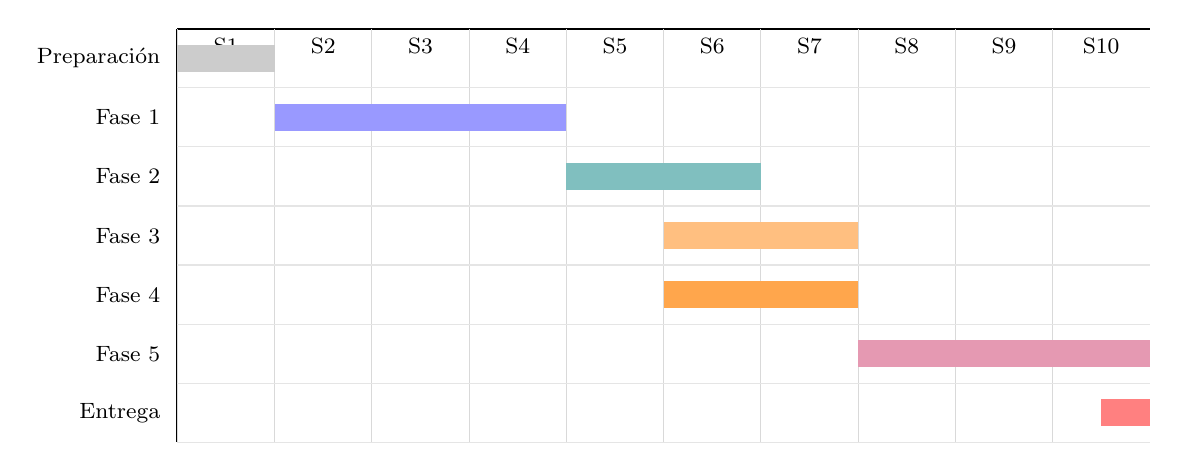
\begin{tikzpicture}[
	bar/.style={fill=#1, draw=#1!70!black, minimum height=0.5cm},
	label/.style={font=\footnotesize, anchor=east},
	xscale=0.95,
	yscale=0.75
]

\def\weekwidth{1.3}
\def\barheight{0.45}

\draw[thick] (0,0) -- (10*\weekwidth,0);
\draw[thick] (0,0) -- (0,-7);

\foreach \i/\w in {0/S1, 1/S2, 2/S3, 3/S4, 4/S5, 5/S6, 6/S7, 7/S8, 8/S9, 9/S10} {
	\node[font=\footnotesize, below] at (\i*\weekwidth + \weekwidth/2, 0) {\w};
	\draw[gray!30] (\i*\weekwidth, 0) -- (\i*\weekwidth, -7);
}

\node[label] at (-0.1, -0.5) {Preparaci\'{o}n};
\fill[gray!40] (0*\weekwidth, -0.5-\barheight/2) rectangle (1*\weekwidth, -0.5+\barheight/2);

\node[label] at (-0.1, -1.5) {Fase 1};
\fill[blue!40] (1*\weekwidth, -1.5-\barheight/2) rectangle (4*\weekwidth, -1.5+\barheight/2);

\node[label] at (-0.1, -2.5) {Fase 2};
\fill[teal!50] (4*\weekwidth, -2.5-\barheight/2) rectangle (6*\weekwidth, -2.5+\barheight/2);

\node[label] at (-0.1, -3.5) {Fase 3};
\fill[orange!50] (5*\weekwidth, -3.5-\barheight/2) rectangle (7*\weekwidth, -3.5+\barheight/2);

\node[label] at (-0.1, -4.5) {Fase 4};
\fill[orange!70] (5*\weekwidth, -4.5-\barheight/2) rectangle (7*\weekwidth, -4.5+\barheight/2);

\node[label] at (-0.1, -5.5) {Fase 5};
\fill[purple!40] (7*\weekwidth, -5.5-\barheight/2) rectangle (10*\weekwidth, -5.5+\barheight/2);

\node[label] at (-0.1, -6.5) {Entrega};
\fill[red!50] (9.5*\weekwidth, -6.5-\barheight/2) rectangle (10*\weekwidth, -6.5+\barheight/2);

\foreach \y in {-1, -2, -3, -4, -5, -6, -7} {
	\draw[gray!20] (0, \y) -- (10*\weekwidth, \y);
}

\end{tikzpicture}
\caption[Diagrama de Gantt]{Diagrama de Gantt del proyecto, mostrando la distribuci\'{o}n temporal de las fases de desarrollo (S1--S10 = semanas 1--10). Fuente: elaboraci\'{o}n propia.}
\label{fig:gantt}
\end{figure}

\section{Resumen de horas por fase}

La Tabla~\ref{tab:horas-fase} resume la distribuci\'{o}n estimada de horas de trabajo por cada fase del proyecto, conforme a la planificaci\'{o}n acordada con el tutor.

\begin{table}[ht]
\centering
\begin{tabular}{l c c}
\hline\hline
Fase & Horas estimadas & Periodo \\ [0.5ex]
\hline
Preparaci\'{o}n & 4 h & S1 \\
Fase 1: An\'{a}lisis y requerimientos & 20 h & S2--S4 \\
Fase 2: Protocolo de comunicaci\'{o}n & 30 h & S4--S6 \\
Fase 3: Adquisici\'{o}n y visualizaci\'{o}n & 22 h & S6--S7 \\
Fase 4: Registro, exportaci\'{o}n y clasificaci\'{o}n & 18 h & S6--S7 \\
Fase 5: Documentaci\'{o}n y entrega final & 32 h & S8--S10 \\
\hline
\textbf{Total} & \textbf{126 h} & \\ \hline
\end{tabular}
\caption[Horas por fase]{Distribuci\'{o}n estimada de horas de trabajo por fase. Fuente: elaboraci\'{o}n propia.}
\label{tab:horas-fase}
\end{table}

\end{document}
